\documentclass[11pt]{scrartcl}
\usepackage{polski}
\usepackage[polish]{babel}

\usepackage{graphicx, float, caption, subcaption}
\usepackage{amsmath}
\usepackage{tabularx}
\graphicspath{{images/}}

\title{Laboratorium 2 - Otoczka wypukła}
\author{Mateusz Podmokły}
\date{18 październik 2023}

\begin{document}
    \maketitle
    \section{Specyfikacja użytego środowiska}
    Specyfikacja:

    \begin{itemize}
        \item Środowisko: Jupyter Notebook,
        \item Język programowania: Python,
        \item System operacyjny: Microsoft Windows 11,
        \item Architektura systemu: x64.
    \end{itemize}
    \section{Przebieg ćwiczenia}

    Ćwiczenie polega na zaimplementowaniu algorytmów Grahama i Jarvisa obliczających
    otoczkę wypukłą oraz na analizie ich wyników.

    \subsection{Losowanie punktów}

    Wylosowane zostały następujące zbiory punktów:

    \begin{enumerate}
        \item 100 losowo wygenerowanych punktów o współrzędnych z przedziału
        \([-100,100]\),
        \item 100 losowo wygenerowanych punktów leżących na okręgu o środku
        \((0,0)\) i promieniu $R=10$,
        \item 100 losowo wygenerowanych punktów leżących na bokach prostokąta
        o wierzchołkach $(-10, 10)$, $(-10,-10)$, $(10,-10)$, $(10,10)$,
        \item punkty na wierzchołkach kwadratu $(0, 0)$, $(10, 0)$, $(10, 10)$,
        $(0, 10)$ oraz punkty wygenerowane losowo w sposób następujący: po 25 punktów na
        dwóch bokach kwadratu leżących na osiach i po 20 punktów na przekątnych kwadratu. 
    \end{enumerate}

    \begin{figure}[H]
        \centering
        \begin{minipage}{0.45\linewidth}
          \centering
          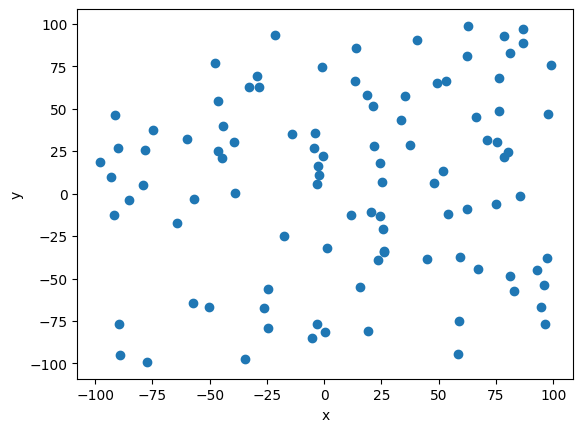
\includegraphics[width=1\linewidth]{2_1.png}
          \caption{Zbiór 1. - obszar kwadratowy.}
        \end{minipage}
        \begin{minipage}{0.45\linewidth}
          \centering
          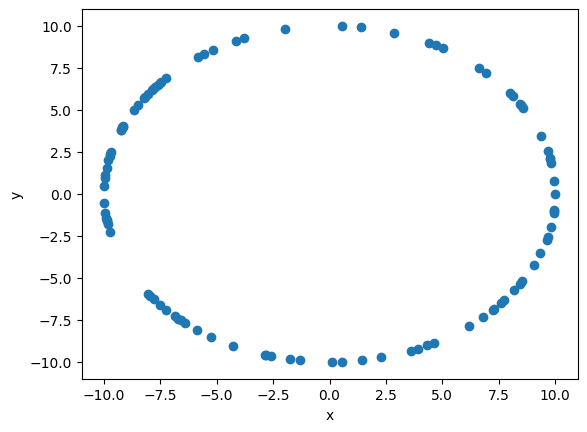
\includegraphics[width=1\linewidth]{2_2.png}
          \caption{Zbiór 2. - okrąg.}
        \end{minipage}
    \end{figure}

    \begin{figure}[H]
        \centering
        \begin{minipage}{0.45\linewidth}
          \centering
          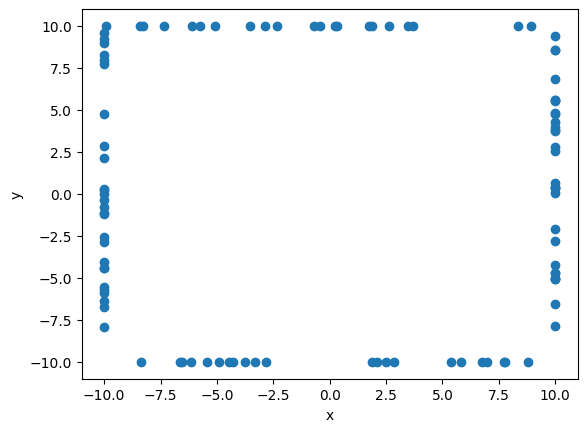
\includegraphics[width=1\linewidth]{2_3.png}
          \caption{Zbiór 3. - boki prostokąta.}
        \end{minipage}
        \begin{minipage}{0.45\linewidth}
          \centering
          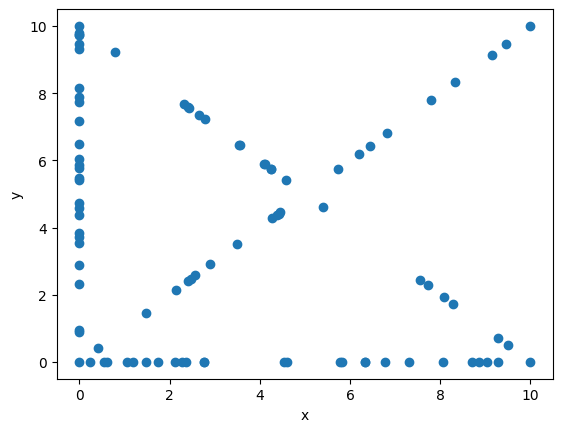
\includegraphics[width=1\linewidth]{2_4.png}
          \caption{Zbiór 4. - boki, wierzchołki i przekątne kwadratu.}
        \end{minipage}
    \end{figure}

    \subsection{Obliczenie otoczki wypukłej}
    Dla każdego zbioru obliczona została otoczka wypukła z użyciem algorytmu
    Grahama oraz algorytmu Jarvisa.

    \section{Analiza wyników}
    \section{Wnioski}
\end{document}